% !TEX program = xelatex
\documentclass[xcolor=dvipsnames, handout, onlymath, 10pt, aspectratio=169]{beamer}
% \usetikzlibrary{positioning, shapes.geometric}


\definecolor{softblue}{RGB}{102,178,255}
\definecolor{softorange}{RGB}{255,204,102}

% WARNING: CORRECTION FOR TEACHING
\newif\ifshow
\showtrue % HACK: Comment out to hide solutions

\usepackage{/Users/gdgarcia/Repos/latex/garcia_commands}

% NOTE: COURSE:
\newcommand{\course}{The fundamentals of data visualization in R}


% NOTE: TOPIC:
\newcommand{\classtopic}{Our topics and goals}

% NOTE: CLASS No:
\newcommand{\classdate}{University of Alberta, Edmonton, May 2025}

% ==========================================
% ==========================================

% NOTE: TITLE SLIDE:
\title{\course}
\subtitle{\classtopic}
\author{Guilherme D.\ Garcia}

\institute[Université Laval] % (optional, but mostly needed)
{
  \mylink{https://gdgarcia.ca}{gdgarcia.ca}\vspace{5ex}
}

\date{\classdate}
\subject{Data analysis}

% ==========================================
% ==========================================

% HACK:: BEGIN

\begin{document}

\selectlanguage{english}
\begin{frame}
	\vspace{2ex}
	\textcolor{lav1}{\noindent\rule{0.66\textwidth}{3pt}}
	\textcolor{lav2}{\noindent\rule{0.33\textwidth}{3pt}}

	\titlepage

	\vfill

	\begin{columns}
		% \begin{column}{0.3\textwidth}
		% 	\begin{flushleft}
		% 		{\includegraphics[height=1.3cm]{/Users/gdgarcia/repos/latex/uni-logos/ULisboa.jpg}}
		% 	\end{flushleft}
		% \end{column}
		\begin{column}{0.5\textwidth}
			\begin{flushleft}
				{\includegraphics[height=1cm]{/Users/gdgarcia/repos/latex/uni-logos/ULaval1.png}}
			\end{flushleft}
		\end{column}
		\begin{column}{0.5\textwidth}
			\begin{flushright}
				{\includegraphics[height=0.6cm]{/Users/gdgarcia/repos/latex/uni-logos/crblm.jpg}}
			\end{flushright}
		\end{column}
	\end{columns}

\end{frame}

\addtobeamertemplate{navigation symbols}{}{%
	\usebeamerfont{footline}%
	\usebeamercolor[fg]{footline}%
	\hspace{1em}%
	\vspace{1ex}%
	{\insertframenumber} of {\inserttotalframenumber}
}



%\setbeamertemplate{background}{\tikz[overlay,remember picture]\node[opacity=0.4, xshift=-1cm, yshift=.8cm] at (current page.south east){\includegraphics[width=.75cm]{/Users/gdgarcia/Dropbox/Academia/Admin/Uni-logos/ULaval2bw.png}};}




% =====================

\begin{frame}{Welcome!}{Why visualize data?}
	\begin{itemize}
		\item \lav{Communicating} results is a key element in research (and in the job market)
		\item Good visuals are a crucial but often underrated skill in academia
		\item[\winner] In some sense, where soft and technical skills meet:
		\item []
	\end{itemize}

	\begin{center}

		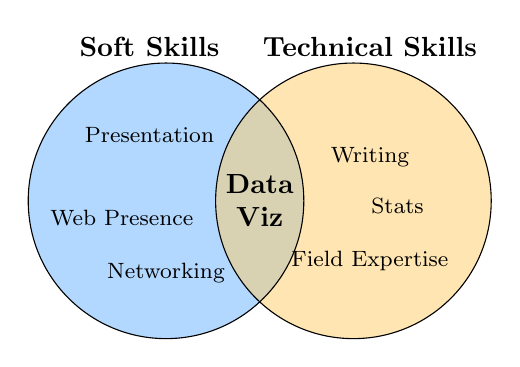
\begin{tikzpicture}[scale=0.7]
			% Define circles
			% Draw filled circles (no blending)
			\fill[softblue, opacity=0.5] (-1.7,0) circle (2.5);
			\fill[softorange, opacity=0.5] (1.7,0) circle (2.5);

			% Draw outlines
			\draw (-1.7,0) circle (2.5);
			\draw (1.7,0) circle (2.5);

			% Titles
			\node at (-2,2.8) {\textbf{Soft Skills}};
			\node at (2,2.8) {\textbf{Technical Skills}};

			% Soft skills content
			\node at (-2,1.2) {\footnotesize Presentation};
			\node at (-2.5,-0.3) {\footnotesize Web Presence};
			\node at (-1.7,-1.3) {\footnotesize Networking};

			% Technical skills content
			\node at (2,0.8) {\footnotesize Writing};
			\node at (2.5,-0.1) {\footnotesize Stats};
			\node at (2,-1.1) {\footnotesize Field Expertise};

			% Overlap label
			\node[align=center, font=\bfseries] at (0,0) {Data\\Viz};

		\end{tikzpicture}


	\end{center}

\end{frame}

% ==========================================
% ==========================================


% =====================
\begin{frame}
	\frametitle{What's a ``good figure"?}
	\framesubtitle{What geoms are being used? What issues do you notice?}

	\begin{figure}
		\begin{center}
			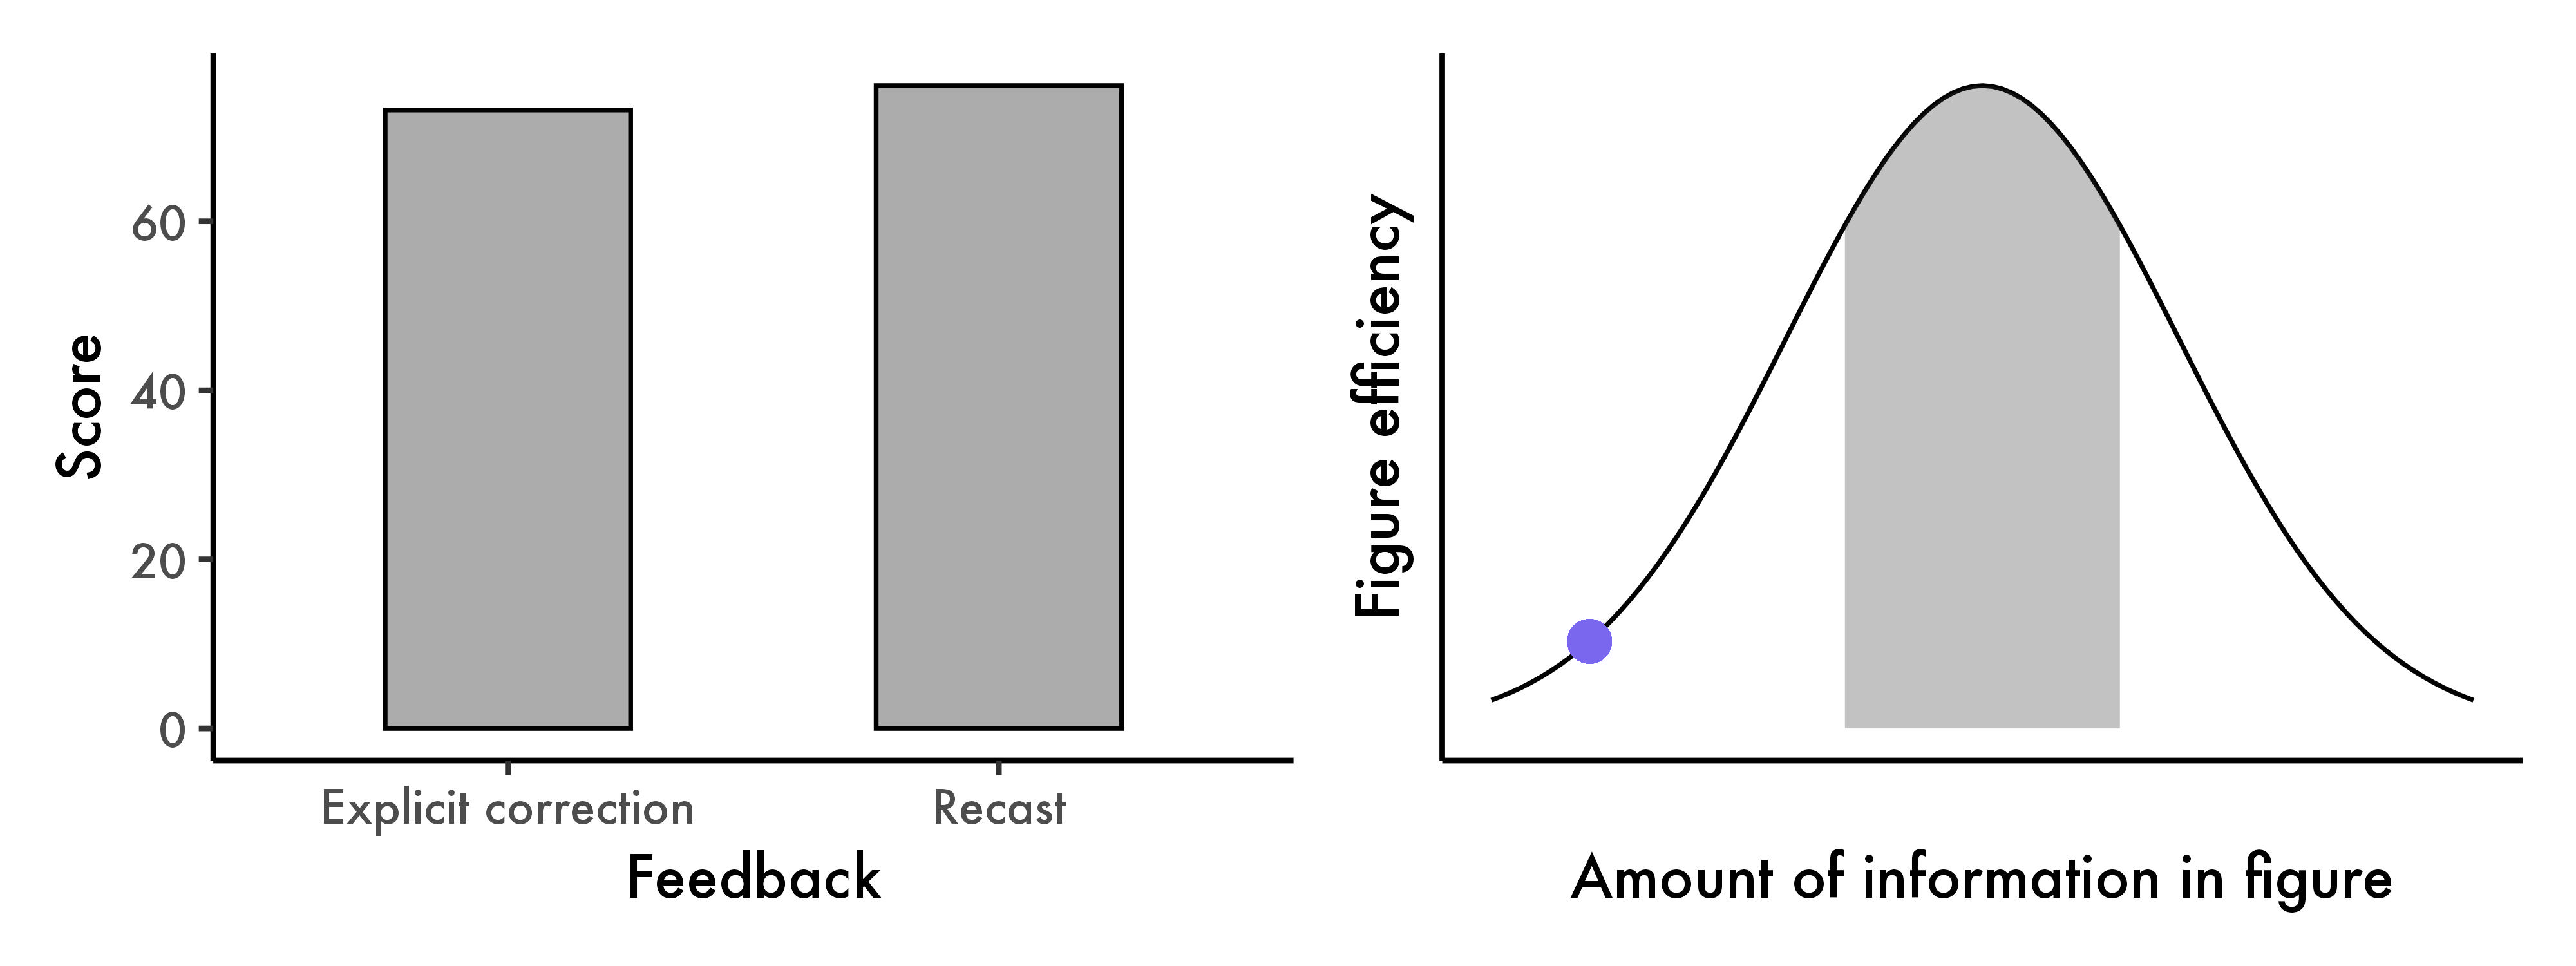
\includegraphics[width=0.95\textwidth]{ex1.jpeg}
		\end{center}
		\caption{Figure vs.\ amount of information}\label{fig:f1}
	\end{figure}

\end{frame}
% =====================

\begin{frame}
	\frametitle{What's a ``good figure"?}
	\framesubtitle{What geoms are being used? What issues do you notice?}

	\begin{figure}
		\begin{center}
			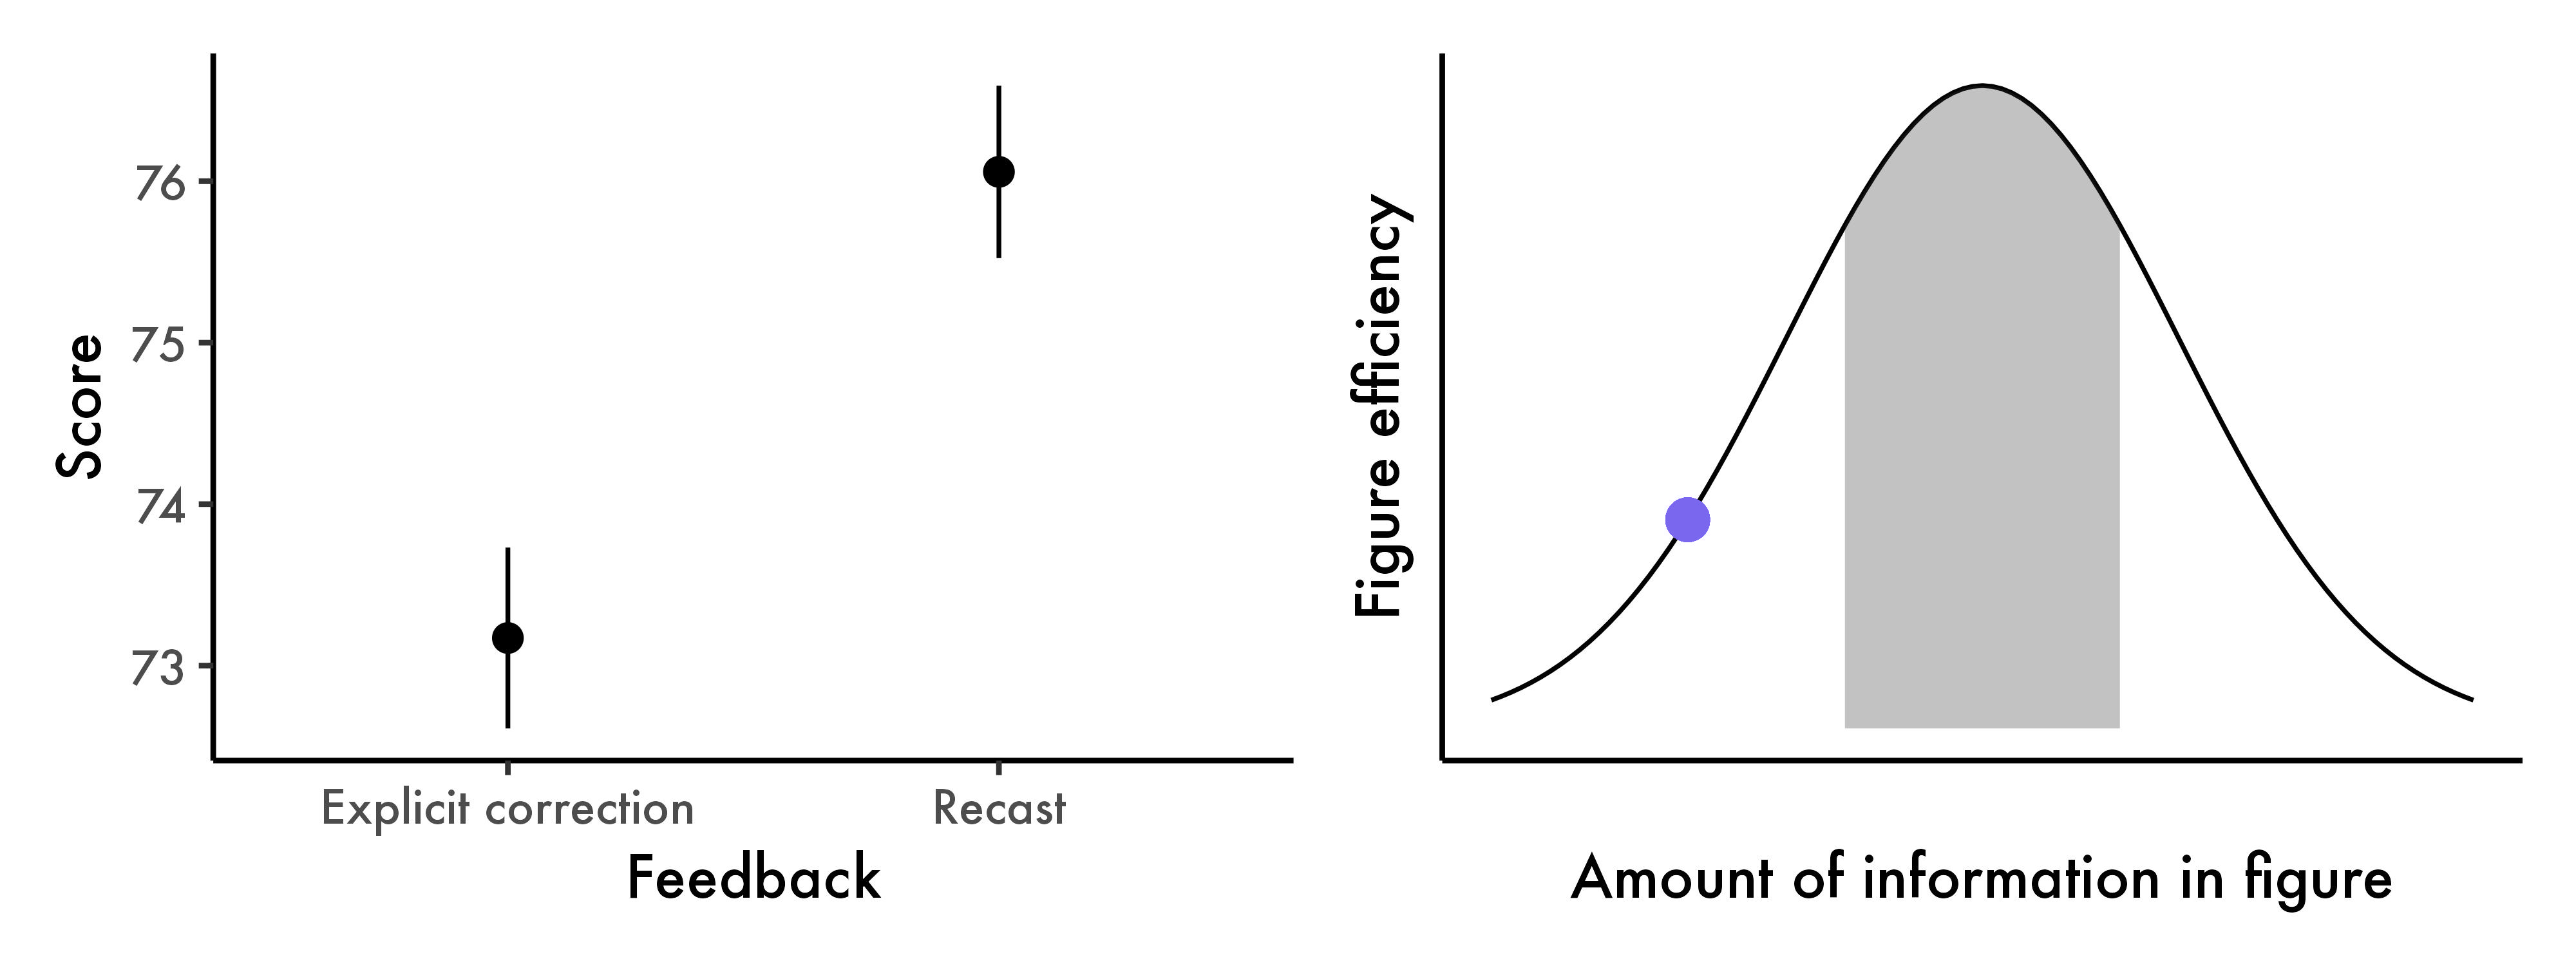
\includegraphics[width=0.95\textwidth]{ex2.jpeg}
		\end{center}
		\caption{Figure vs.\ amount of information}\label{fig:f2}
	\end{figure}

\end{frame}
% =====================

\begin{frame}
	\frametitle{What's a ``good figure"?}
	\framesubtitle{What geoms are being used? What issues do you notice?}

	\begin{figure}
		\begin{center}
			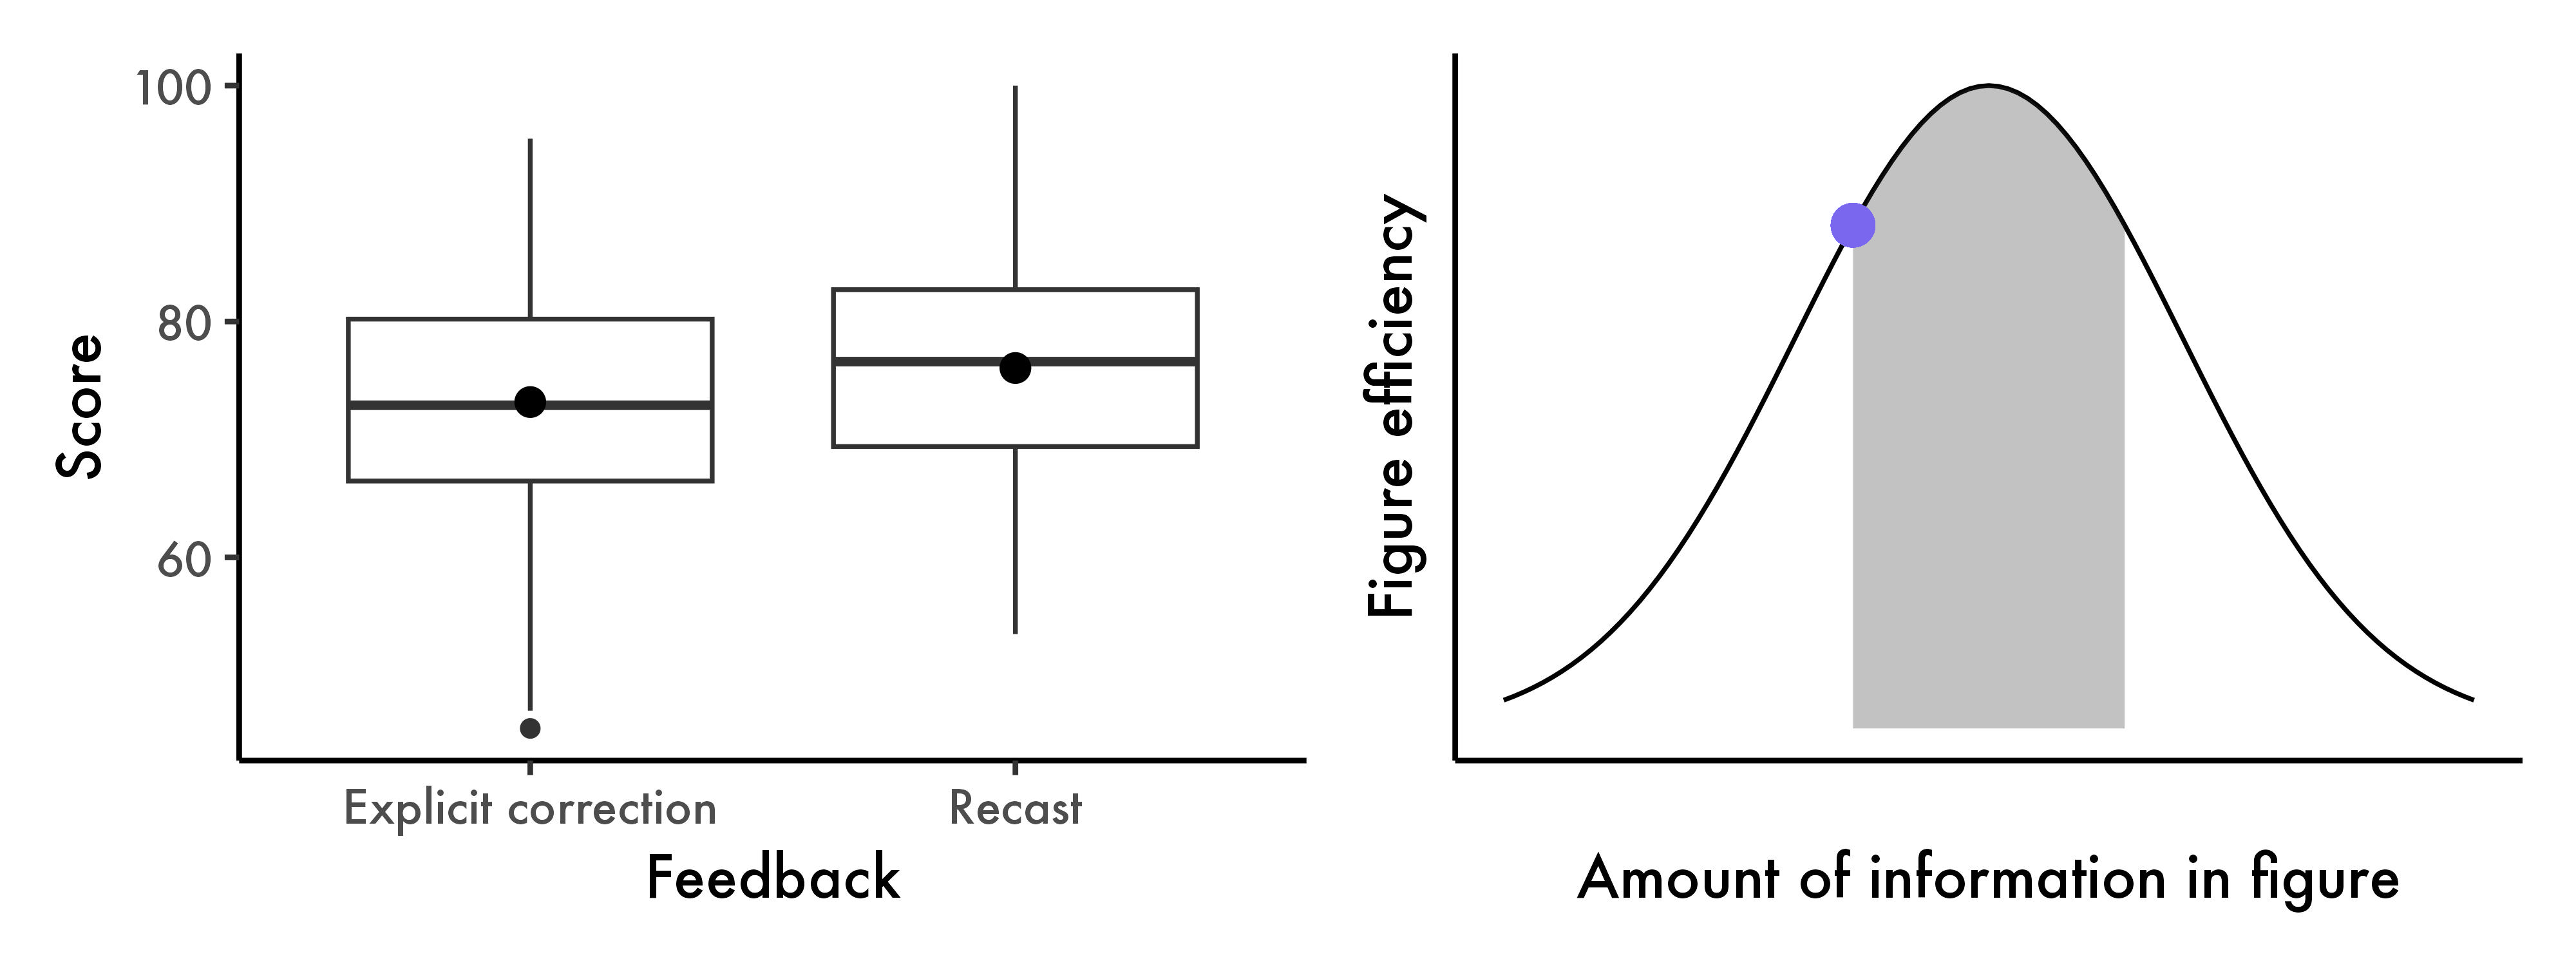
\includegraphics[width=0.95\textwidth]{ex3.jpeg}
		\end{center}
		\caption{Figure vs.\ amount of information}\label{fig:f3}
	\end{figure}

\end{frame}
% =====================

\begin{frame}
	\frametitle{What's a ``good figure"?}
	\framesubtitle{What geoms are being used? What issues do you notice?}

	\begin{figure}
		\begin{center}
			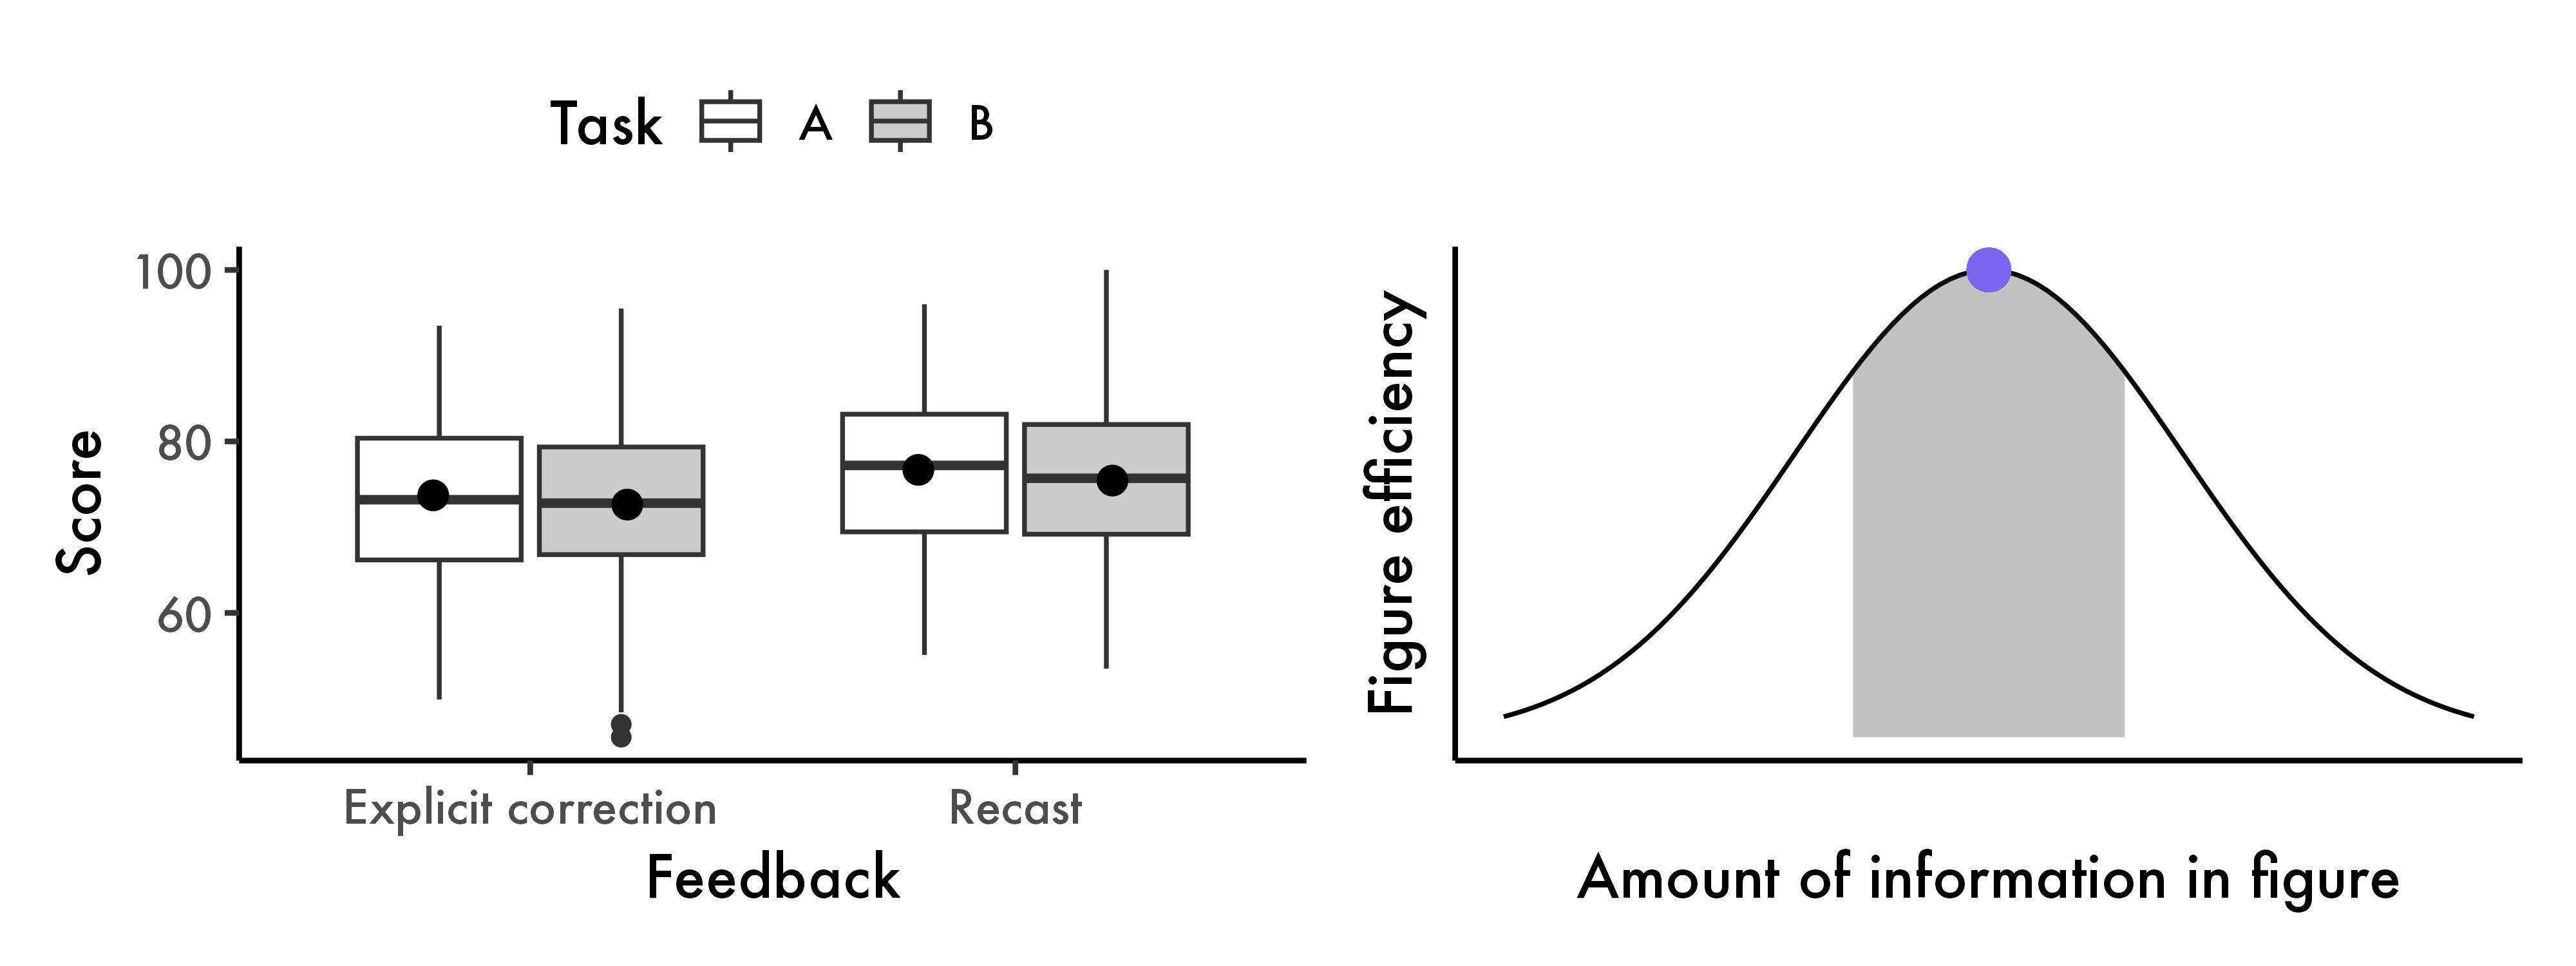
\includegraphics[width=0.95\textwidth]{ex4.jpeg}
		\end{center}
		\caption{Figure vs.\ amount of information}\label{fig:f4}
	\end{figure}

\end{frame}
% =====================

\begin{frame}
	\frametitle{What's a ``good figure"?}
	\framesubtitle{What geoms are being used? What issues do you notice?}

	\begin{figure}
		\begin{center}
			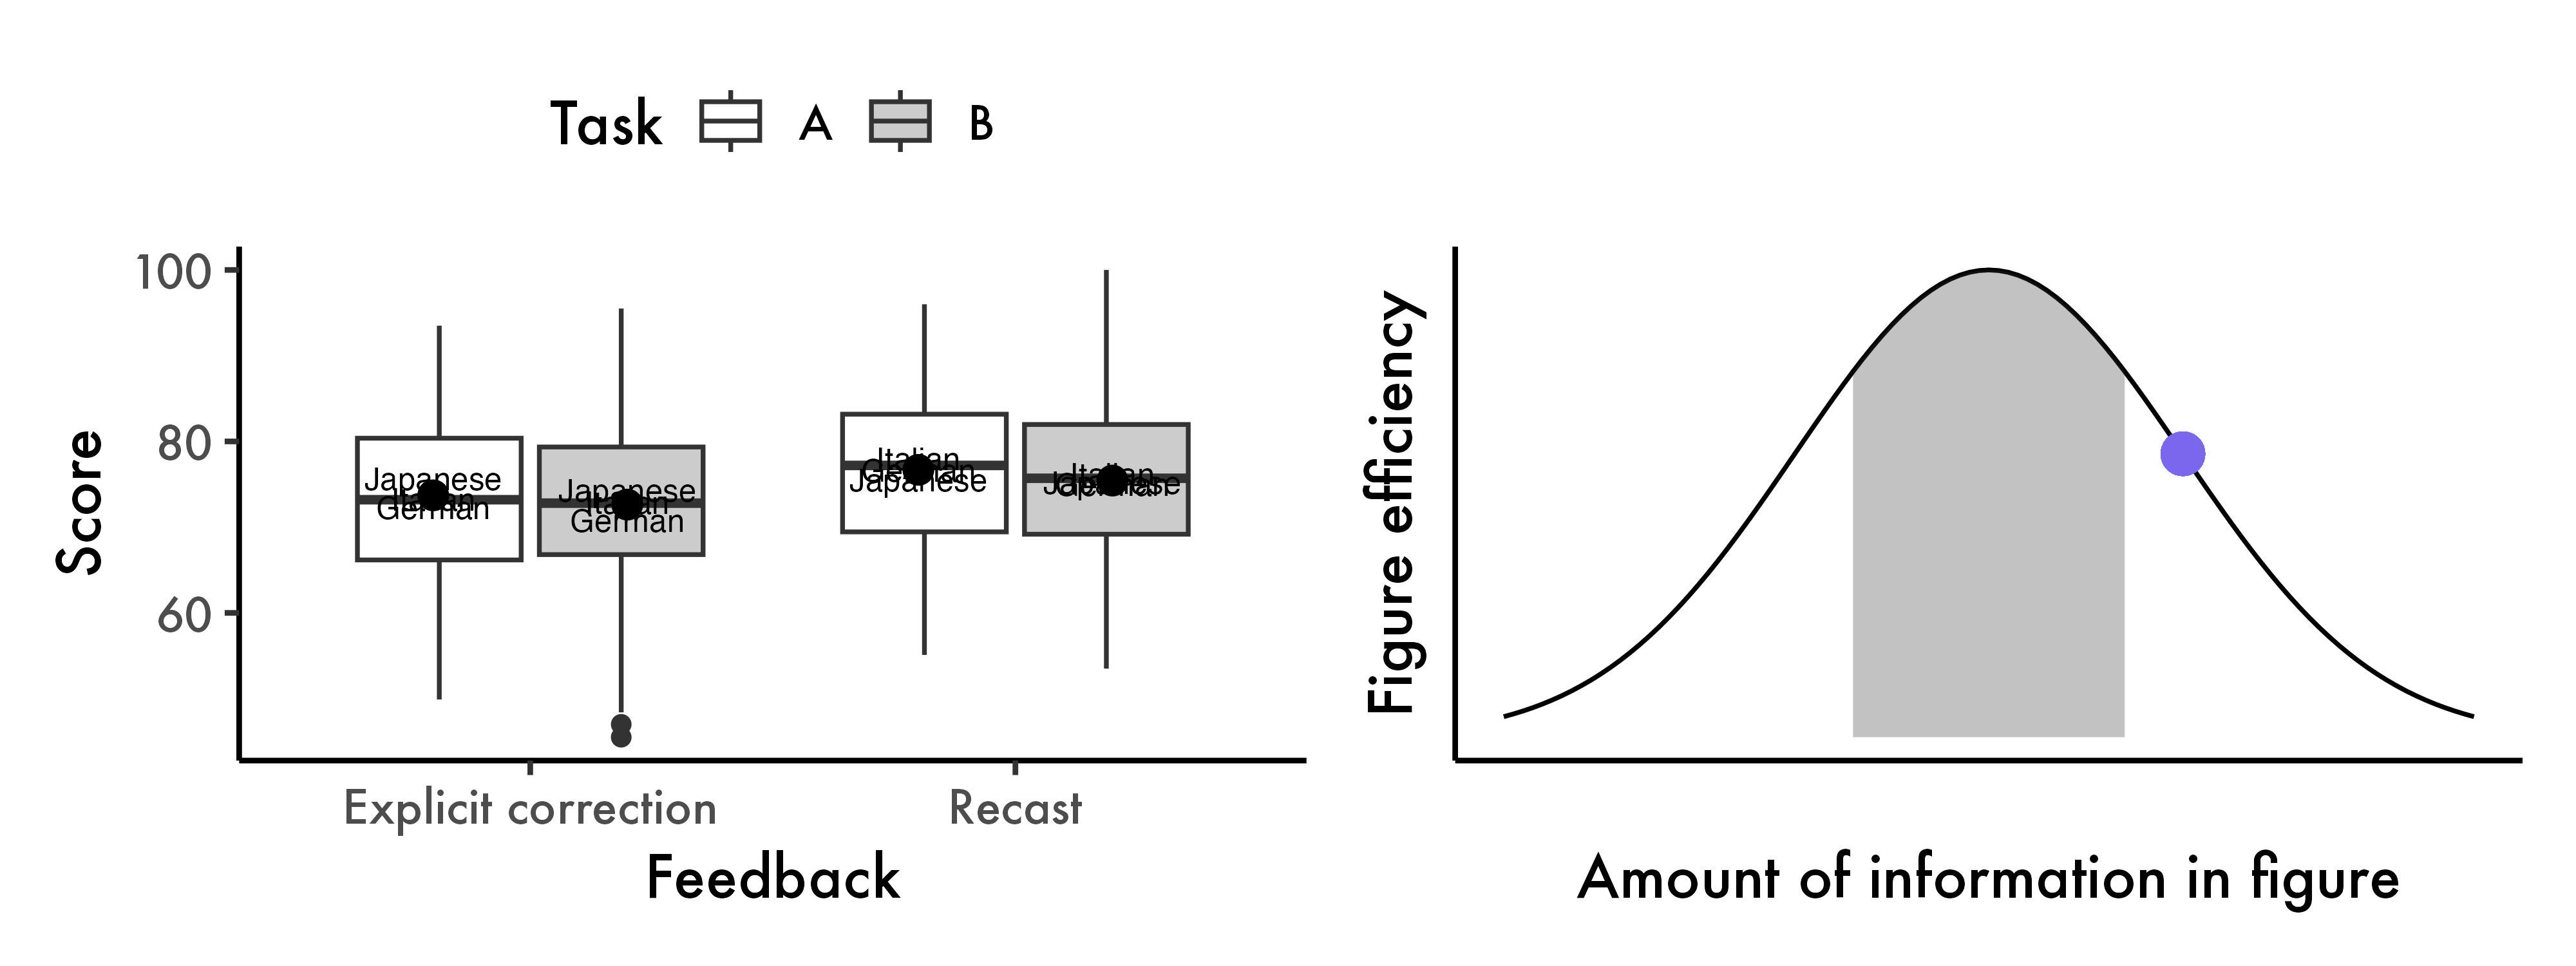
\includegraphics[width=0.95\textwidth]{ex5.jpeg}
		\end{center}
		\caption{Figure vs.\ amount of information}\label{fig:f5}
	\end{figure}

\end{frame}

% =====================
%


% =====================
\begin{frame}
	\frametitle{What's a ``good figure"?}
	\framesubtitle{Form also matters}

	\begin{figure}
		\begin{center}
			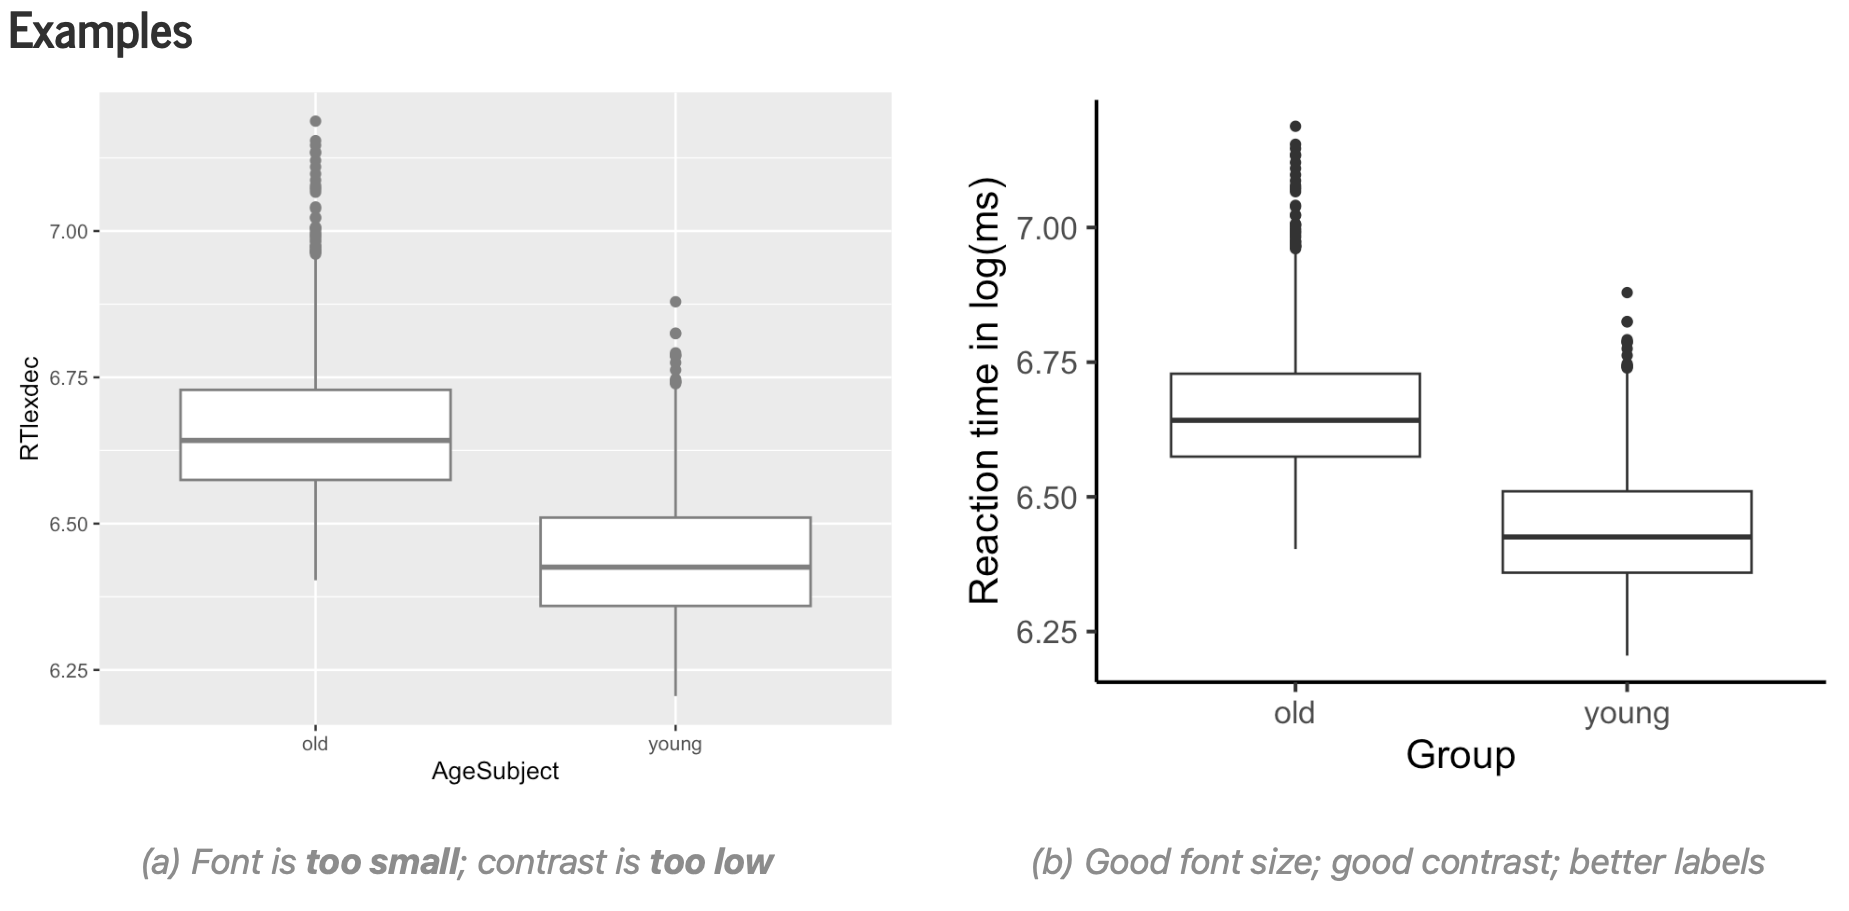
\includegraphics[width=0.8\textwidth]{slr_figures_1.png}
		\end{center}
		\caption{From the guidelines at SLR (1)}\label{fig:slr1}
	\end{figure}

\end{frame}
% =====================

\begin{frame}
	\frametitle{What's a ``good figure"?}
	\framesubtitle{Form also matters}

	\begin{figure}
		\begin{center}
			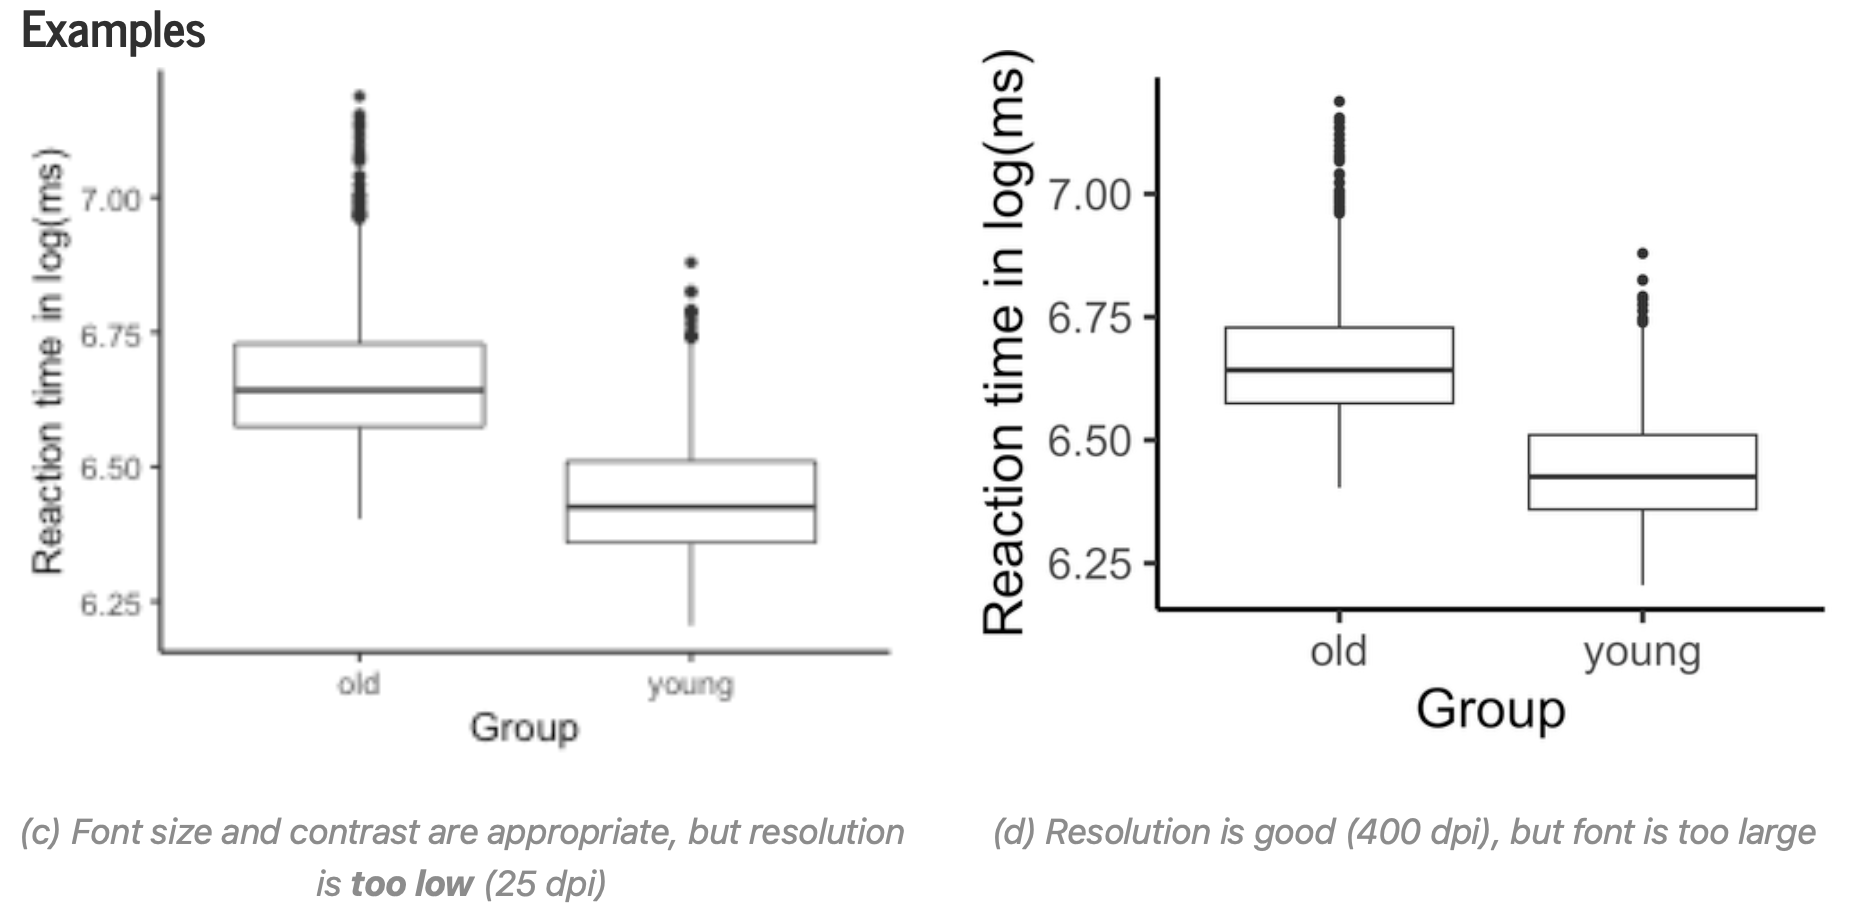
\includegraphics[width=0.8\textwidth]{slr_figures_2.png}
		\end{center}
		\caption{From the guidelines at SLR (2)}\label{fig:slr2}
	\end{figure}

\end{frame}

% =====================
\begin{frame}
	\frametitle{Our itinerary}
	\framesubtitle{Topics we will cover in three days}

	% \begin{columns}
	% 	\begin{column}{0.7\textwidth}
	\begin{enumerate}
		\itemsep=0.5pt
		\item \lav{Basic principles behind data visualization}
		\item [] Data cleaning/preparation; \var{ggplot2} and its core structure; essential \var{geoms}
		\item [] \hl{Practice}
		\item []
		\item \lav{Data transformation for visualization}
		\item [] Scales, facets, and grids; aesthetics; \var{dplyr} and conditionals
		\item [] \hl{Practice}
		\item []
		\item \lav{Plotting individual variation}
		\item [] Visualizing model estimates; a brief intro to Quarto
		\item [] Interactive plots and extra packages
		\item[] \hl{Practice}
	\end{enumerate}
	% \end{column}
	% \begin{column}{0.4\textwidth}
	% 	\begin{center}
	% 		% {
\includegraphics[width=0.7\textwidth]{cover.jpg}}
	% 	\end{center}
	% \end{column}
	%
	% \end{columns}


\end{frame}
% =====================


% =====================

% =====================


% =====================
\begin{frame}
	\frametitle{Materials and logistics}
	\framesubtitle{}

	\begin{itemize}
		\item[\winner] \textbf{IDE:} many options (\textbf{Positron}, RStudio, Sublime, VSCode, nvim, etc.)
		\item If you prefer, you can also use \mylink{http://posit.cloud}{posit.cloud}
		\item We will focus on \hl{scripts}, \textit{not} slides
		\item Our main package will be \var{tidyverse}, but we will certainly use others \smallCite{\citealt{tidyverse}}
		\item[] \lav{What you need:} an IDE + \var{tidyverse} installed
	\end{itemize}


	\begin{importanttitle}{Positron vs.\ RStudio}
		\begin{itemize}
			\item Positron is the new IDE from Posit, and will likely replace RStudio
			\item So you might as well switch to Positron these days
			\item [\winner] It's a personal choice: for our course, it won't matter which IDE you use
		\end{itemize}
	\end{importanttitle}


\end{frame}
% =====================


% =====================
\begin{frame}{Survey}{\mylink{https://forms.cloud.microsoft/r/m6mCwa4d5m}{forms.cloud.microsoft/r/m6mCwa4d5m}}

	\begin{figure}
		\begin{center}
			
\includegraphics[width=0.4\textwidth]{qr.png}
		\end{center}
		% \caption{}\label{fig:}
	\end{figure}

\end{frame}
% =====================


% =====================
% =====================
% ==========================================
% ==========================================

\begin{frame}[allowframebreaks=0.7]

	{
		\footnotesize

		\frametitle{References}
		\bibliographystyle{apalike}
		\bibliography{/Users/gdgarcia/Repos/latex/references}

	}

\end{frame}

\end{document}
